\section{Arrizal Furqona Gifary(1174070)}
\subsection{Membaca Shapefile dengan PySHP}
\begin{enumerate}
	\item Nomor 1
	\lstinputlisting{src/tugas3/1174070/soal1.py}
	\begin{figure}[H]
		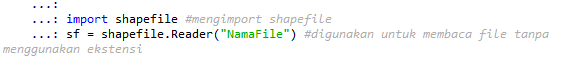
\includegraphics[width=6cm]{figures/Tugas3/1174070/soal1.png}
		\centering
		\caption{Gambar Soal 1}
	\end{figure}
	\item Nomor 2
	\lstinputlisting{src/tugas3/1174070/soal2.py}
	\begin{figure}[H]
		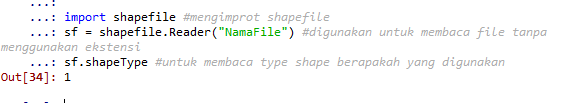
\includegraphics[width=6cm]{figures/Tugas3/1174070/soal2.png}
		\centering
		\caption{Gambar Soal 2)}
	\end{figure}
	\item Nomor 3
	\lstinputlisting{src/tugas3/1174070/soal3.py}
	\begin{figure}[H]
		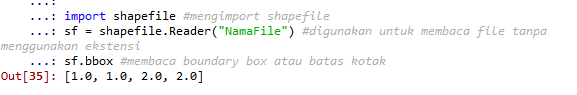
\includegraphics[width=6cm]{figures/Tugas3/1174070/soal3.png}
		\centering
		\caption{Gambar Soal 3}
	\end{figure}
	\item Nomor 4
	\lstinputlisting{src/tugas3/1174070/soal4.py}
	\begin{figure}[H]
		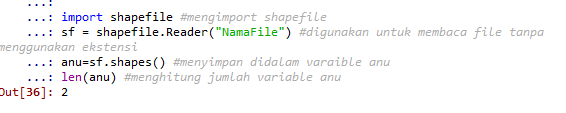
\includegraphics[width=6cm]{figures/Tugas3/1174070/soal4.png}
		\centering
		\caption{Gambar Soal 4}
	\end{figure}
	\item Nomor 5
	\lstinputlisting{src/tugas3/1174070/soal5.py}
	\begin{figure}[H]
		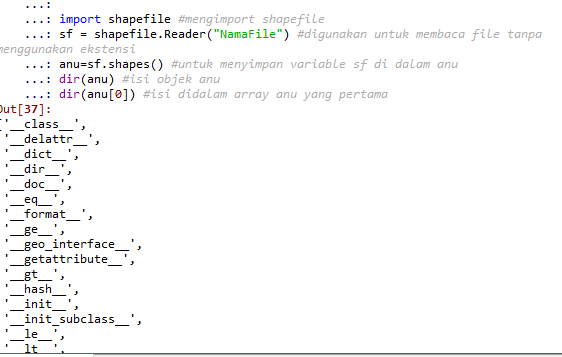
\includegraphics[width=6cm]{figures/Tugas3/1174070/soal5.png}
		\centering
		\caption{Gambar Soal 5)}
	\end{figure}
	\item Nomor 6
	\lstinputlisting{src/tugas3/1174070/soal6.py}
	\begin{figure}[H]
		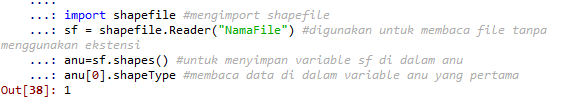
\includegraphics[width=6cm]{figures/Tugas3/1174070/soal6.png}
		\centering
		\caption{Gambar Soal 6}
	\end{figure}
	\item Nomor 7
	\lstinputlisting{src/tugas3/1174070/soal7.py}
	\begin{figure}[H]
		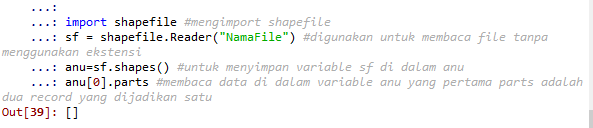
\includegraphics[width=6cm]{figures/Tugas3/1174070/soal7.png}
		\centering
		\caption{Gambar Soal 7)}
	\end{figure}
	\item Nomor 8
	\lstinputlisting{src/tugas3/1174070/soal8.py}
	\begin{figure}[H]
		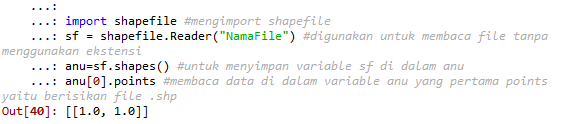
\includegraphics[width=6cm]{figures/Tugas3/1174070/soal8.png}
		\centering
		\caption{Gambar Soal 8)}
	\end{figure}
	\item Nomor 9
	\lstinputlisting{src/tugas3/1174070/soal9.py}
	\begin{figure}[H]
		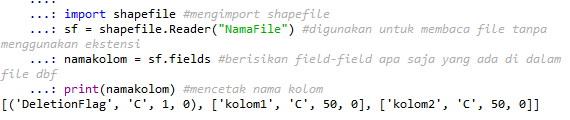
\includegraphics[width=6cm]{figures/Tugas3/1174070/soal9.png}
		\centering
		\caption{Gambar Soal 9}
	\end{figure}
	\item Nomor 10
	\lstinputlisting{src/tugas3/1174070/soal10.py}
	\begin{figure}[H]
		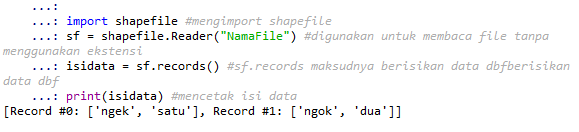
\includegraphics[width=6cm]{figures/Tugas3/1174070/soal10.png}
		\centering
		\caption{Gambar Soal 10 }
	\end{figure}
	\item Nomor 11
	\lstinputlisting{src/tugas3/1174070/soal11.py}
	\begin{figure}[H]
		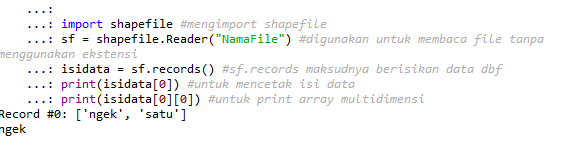
\includegraphics[width=6cm]{figures/Tugas3/1174070/soal11.png}
		\centering
		\caption{Gambar Soal 11 }
	\end{figure}
\end{enumerate}
\subsection{Link}
\verb|https://youtu.be/PNHW_7Yi6IM|
